Mixing features in Traverso \Version\ currently include gain, panorama, different fade shapes for fade-in and -out, trimming, splitting, moving of audio clips, and gain curves. An infrastructure for effect plugins using the LV2 standard is implemented, but  the LV2 standard and plugins are still under heavy construction. Traverso also has basic support for using Sox to process audio clips.

\section{Moving, trimming, splitting}
Clips can be moved freely by holding \hact{D} and moving the mouse. If snapping is active (\sact{S~N}), both ends of the dragged clip will snap to the beginning of the sheet, edges of other clips, markers, and to the work cursor.

Move the mouse cursor on a clip, hold \hact{E}, and move the mouse horizontally to drag the edge of the clip which is nearest to the mouse position. If snapping is active, the edge will snap to the positions described above.

Audio clips can be split by pointing the mouse cursor to the desired position and pressing \sact{X}. Of course the edges of the two clip fragments can be fine-tuned by holding \hact{E} as describes above.

\section{Fades}
Both ends of a clip can be faded smoothly by holding \hact{F} on the left or right half of the clip and moving the mouse horizontally. On the left half the key action refers to the fade-in, on the right half it refers to the fade-out. Several fade shapes are available, which can be toggled by \sact{M} (\FigB~\ref{fig_fades01}).

\begin{figure}[t]
 \centering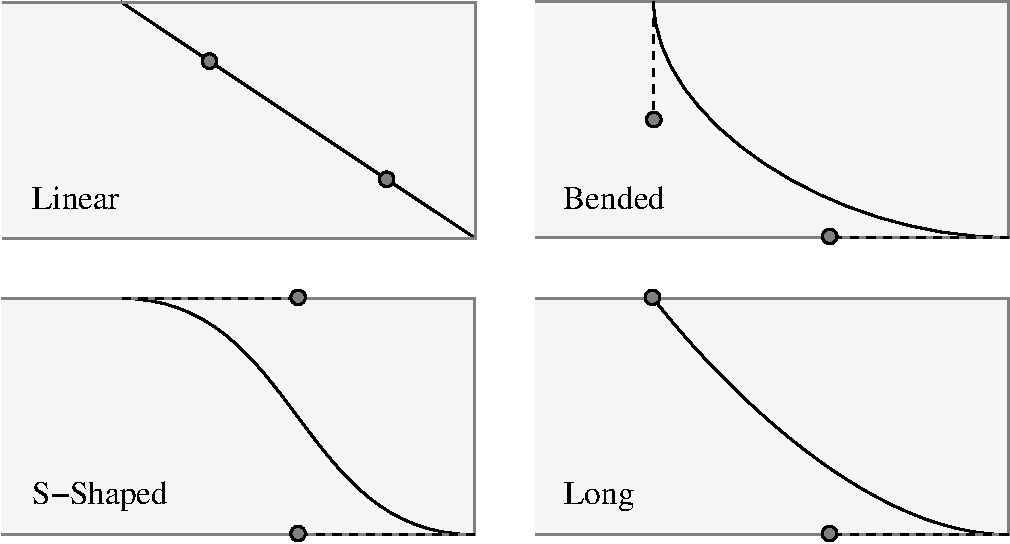
\includegraphics[width=0.8\textwidth]{../images/fades}
 \caption{Different fade shapes are available in Traverso. Fade curves are defined as splines with two control points (circles) which can be modified by the values ``bending'' and ``strength''.}
 \label{fig_fades01}
\end{figure}

All shapes are based on a cubic spline curve with four knots. Two knots define the bending of the non-linear shapes. The positions of these control knots can be modified by two values ``bending'' and ``strength''. ``Bending'' defines the direction of the tangent in the end point, whereas ``strength'' changes the weight of the tangent (\FigB~\ref{fig_fades02}). It is not possible to move the control knots freely and independently, instead Traverso knows several modes which are relevant for fade shapes (\FigB~\ref{fig_fades01}):

\begin{figure}[t]
 \centering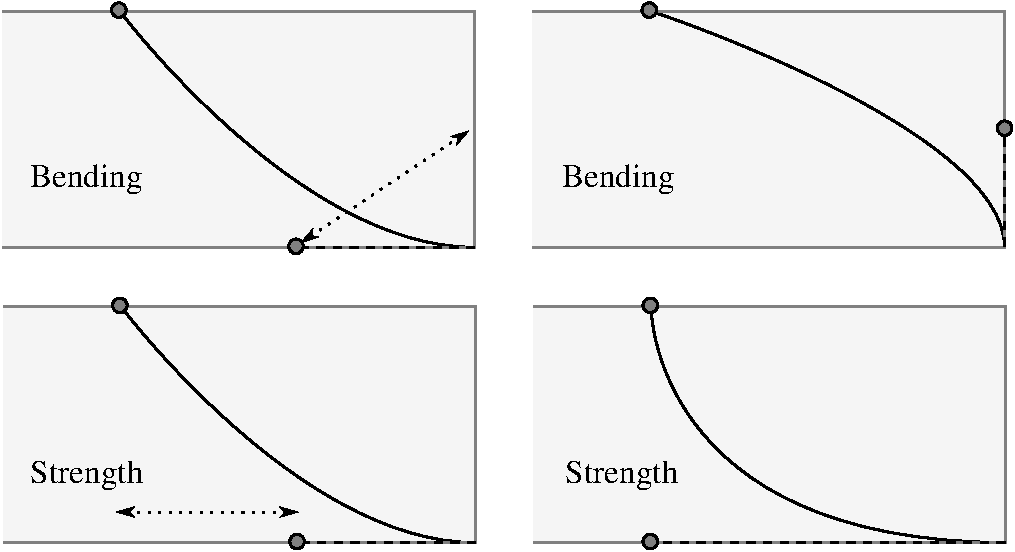
\includegraphics[width=0.8\textwidth]{../images/fades2}
 \caption{Bending and strength values can be used to alter the shape of the fade curves. (Demonstrated with the ``Long'' mode.)}
 \label{fig_fades02}
\end{figure}

\subsection{Linear}
Linear fades are a straight line between the start and end point. The control knots can't be changed. Linear fades tend to sound rather abrupt at the low-level end of the fade, and are thus not the preferred mode for long fade-outs, e.\,g. at the end of a sheet.

\subsection{S-shaped}
The S-shaped mode starts with a horizontal tangent, is steep a the center, and passes into a horizontal tangent again. The beginning and end are very smooth, but the center part can sometimes change too quickly in short S-fades. The ``strength'' parameter can be used to soften the center part and make the volume change less obvious. The ``bending'' factor should usually remain between linear and horizontal tangents, however, vertical tangents can be used for effects.

\subsection{Bended}
The bended mode acts similar to the S-shaped mode, but the control knots point to the same side. This mode can be used to achieve a very fast volume drop at the beginning of the fade-out, and very soft towards the end. Both control parameters are useful to find the best balance between a beginning that is not too fast, and an ending that is still slow enough for a soft fade-out effect.

\subsection{Long}
The long mode only allows to change the control knot at the low-level end of the fade. This mode is often used for very smooth fade-outs, e.\,g. at the end of a sheet. The high-level end changes fastly, but the low-level tail is very soft. The long mode often sounds more musical than a similar bended mode.

The fades can be edited numerically by pressing \sact{E} on a clip, and changing to the page ``Fades'' in the clip settings dialog.

\section{Gain curve}
Gain curves are a powerful feature to change the gain of an audio clip in the time line. The curves are child elements of audio clips, therefore their \emph{relative} position to the audio clip will always stays the same. To change to effects mode, select the entry ``Mode: Effects'' from the dropdown menu in the menu bar (\FigB~\ref{fig_gcurve01}). To change back to edit mode ``Mode: Edit''. A default curve node is added automatically at the beginning of the clip at 0~dB. Additional nodes can be created by \dact{C} at the position of the mouse cursor. Nodes can also be dragged (\hact{D}) and removed (\dact{R}). These actions always apply to the node closest to the mouse cursor, which is indicated by a different colour.

\begin{figure}[t]
 \centering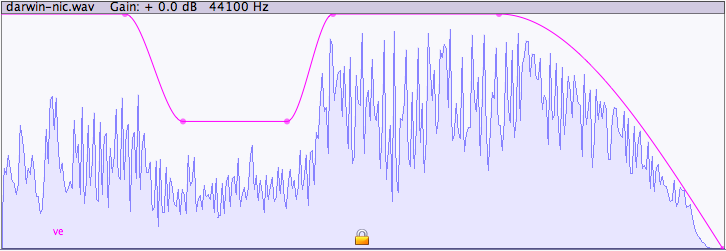
\includegraphics[width=\textwidth]{../images/gcurve01}
 \caption{The ``effects mode'' of Traverso can be activated from the dropdown menu in the menu bar. Gain curves are only visible in that mode. Nodes can be added, removed, and dragged freely.}
 \label{fig_gcurve01}
\end{figure}

\section{Plugins}
Traverso supports the LV2 plugin interface, which is the successor of the LADSPA standard. Plugins can be added to tracks by pressing \sact{F5}, which opens a list of all LV2 plugins installed on the system (\FigB~\ref{fig_pluglist}). Active plugins will be shown as semi-transparent fields in the track view. These fields have their own context menu; just try it out by holding the mouse on them and pressing \sact{Q} or \sact{Right Mouse Button}. Pressing \sact{E} will open a generic dialog, which allows to adjust the plugin parameters. Plugins can also be bypassed (\sact{B}) and removed (\dact{R}). Version 0.40.x inserts all plugins post-fader. More flexible solutions will follow in upcoming versions.

\begin{figure}[t]
 \centering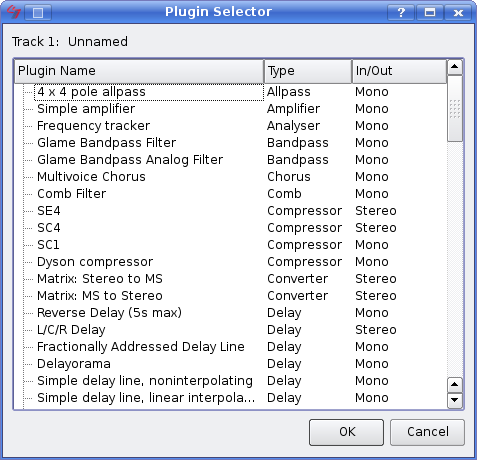
\includegraphics[width=0.6\textwidth]{../images/plugin-list}
 \caption{Plugins can be added to a track by pressing \sact{F5}.}
 \label{fig_pluglist}
\end{figure}


